%\usepackage {pdfsync} 

%\begin{document}
\section{Turbulent flow}
\subsection{Definition of turbulence}
\begin{itemize}
   \item Unpredictable, small perturbation grows too fast as to render impossible for deterministic prediction.
   \item Increased mixing, mix much faster than molecular diffusion.
   \item Wide range of spatial wave lengths.
\end{itemize}
% Turbulence_in_Fluids_4ed_Lesieur
Velocities: $u$ longitudinal, $v$ transverse, $w$ spanwise.
 
\section{Linear-Instability Theory}
\subsection{Orr-Sommerfeld equation}
Linearized Navier-Stokes equation with the condition (uniform $\rho$ and mean flow field $(\bar{u}(y),0,0)$), and use \emph{normal mode analysis} (waveform for the perturbation) to obtain the Orr-Sommerfeld equation. 
Special condition of Orr-Sommerfeld gives the Rayleigh equation (2D inviscid) and Kuo equation (2D rotation).
\subsubsection{Normal mode analysis}
The analysis is done by inserting wave form solution of the perturbation (e.g., velocity, streamfunction, etc) to obtain instability criterions for the equations that result in a positive complex growth rate $\omega_i= \alpha c_i>0$.
The variables involved in the criterions include the mean background flow, perturbed wavenumber, Reynolds number, Coriolis parameter etc.
\begin{itemize}
\subsubsection{Rayleigh equation (2D, $\nu=0$)}
   \item{Rayleigh instability criterion}: An inflection point must exist in the flow ($\bar{u}''$ change sign).
   \item{Fjortoft instability criterion (sufficient condition)}: The absolute vorticity $|du/dy|$ must reach maximum at the inflection point (see figure (d)).
      \begin{figure}[H]
         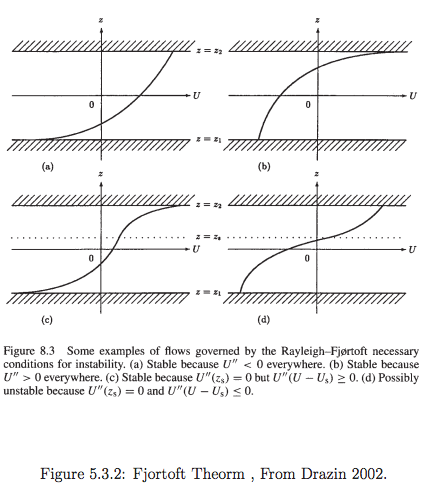
\includegraphics[width=0.5\textwidth]{FjortoftThm}
      \end{figure}
\end{itemize}
notice figure (c) has inflection, but vorticity goes to zero at inflection point, which kills the instability.
 
\subsubsection{Kuo equation (with rotational $\beta$-plane)}
Instability criterion: $\bar{u}''-\frac{df}{dy}$ must change sign.

\subsubsection{3D Orr-Sommerfeld equation}
Dependence of velocity perturbation growth rate $\omega_i$ (imaginery part of angular frequency) on Reynolds number ($Re= \frac{UL}{\nu}$) and wavenumber.
\begin{figure}[H]
   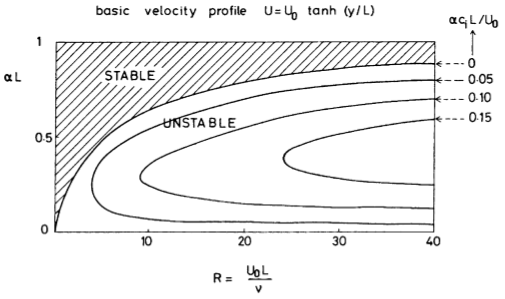
\includegraphics[width=0.5\textwidth]{3d_Instability}
\end{figure} 





\section{Moments, Homogeneity, and Stationarity}
\begin{itemize}
   \item{Moments}: ``n"th order moment is the ensemble average of any tensorial product of $n$-components of the velocity field 
   \item{Homogeneity}: Invariant of any mean quantity after translation over space.
   \item{Stationarity}: Invariant of any mean quantity after translation over time.
   \item{Isotropy}: Invariant of any mean quantity after simultaneous rotation of the set of $n$ points.
\end{itemize}
\subsection{Ensemble average}
An experiment gives a single realization of a set of ($n \times m$)-point $(x_i,t_j)$ solution $u(x_i,t_j)$.
When given an ensemble of $N$ realizations one could define the enbsemble average operator $\left< \cdot \right>$ applied over the set of random variables, e.g.,

\begin{equation}
   \left< u(x_1,t_1) u(x_2,t_2) \dotsc u(x_n,t_n) \right> = \lim_{\substack{N \rightarrow \infty}}\frac{1}{N}\sum\limits^N_{i=1} u^i(x_1,t_1)u^i(x_2,t_2)\dotsc u^i(x_n,t_n)
\end{equation}
Above is the $n$th moment of the velocity.

\subsection{Homogeneity}
\subsubsection{Definition} Invariant of the mean quantity after tranlation over space (i.e., uniform in space),

\begin{equation}
   \left< u_{\alpha_1}(x_1,t_1) u_{\alpha_2}(x_2,t_2) \dotsc u_{\alpha_n}(x_n,t_n) \right> = \left< u_{\alpha_1}(x_1+r,t_1) u_{\alpha_2}(x_2+r,t_2) \dotsc u_{\alpha_n}(x_n+r,t_n) \right>
\end{equation}
where $\alpha_i$ is the index of the coordinate (e.g., $\vec{u}=(u,v,w)$).
For instance, the velocity correlation between two spatial points $x_1$ and $x_1+r$ at $t_1$ and $t_2$, respectively, denoted as a tensorised correlation matrix
\begin{equation}
   [(u(x_1,t_1))^i, (v(x_1,t_1))^i] [(u(x_1+r,t_2))^i, (v(x_1+r,t_2))^i]^T = 
   \left( 
   \begin{array}{cc}
      \left<u(x_1,t_1)u(x_1+r,t_2)\right> & \left<u(x_1,t_1)v(x_1+r,t_2)\right> \\
      \left<v(x_1,t_1)u(x_1+r,t_2)\right> & \left<v(x_1,t_1)v(x_1+r,t_2)\right>
   \end{array}
   \right),
\end{equation}
shorthanded as
\begin{equation}
   U_{ij}(r,t_1,t_2) = \left< u_i(x_1,t_1)u_j(x_1+r,t_2) \right>.
\end{equation}

\subsubsection{Remarks} 
\begin{enumerate}
   \item For homogeneous turbulence, any mean quantity is invariant with a translation of the spatial points (i.e., mean quantity is homogeneous in space). 
         e.g., the mean velocity $\left< u(x,t) \right>$ is independent of x (i.e., mean velocity is homogeneous in space).
   \item An ergodic hypothesis allows one to calculate enesemble average $\left< \cdot \right>$ as a spatial average 
         \begin{equation}
            U_{ij}(r,t_1,t_2) = \lim_{\substack V \rightarrow \infty} \frac{1}{V}\int_V u_i(x_1,t_1)u_j(x_1+r,t_2) dx_1,
         \end{equation}
         essentially using one realization assuming spatial indices as the ensemble indices.
         Therefore, the correlation between the two points, $x_1$ and $x_1+r$, averaged over all realizations is the same as spatially averaging between all pairs of points $x_i$ and $x_i+r$.
\end{enumerate}
\subsection{Stationarity} 
\subsubsection{Definition} Invariant of the mean quantity after tranlation over time,

\begin{equation}
   \left< u_{\alpha_1}(x_1,t_1) u_{\alpha_2}(x_2,t_2) \dotsc u_{\alpha_n}(x_n,t_n) \right> = \left< u_{\alpha_1}(x_1,t_1+\tau) u_{\alpha_2}(x_2,t_2+\tau) \dotsc u_{\alpha_n}(x_n,t_n+\tau) \right>
\end{equation}

\subsubsection{Remarks} An ergodic hypothesis allows one to calculate enesemble average as a time average
         \begin{equation}
            U_{ij}(x_1,x_2,\tau) = \lim_{\substack T \rightarrow \infty} \frac{1}{T}\int_T u_i(x_1,t_1)u_j(x_2,t_1+\tau) dt_1,
         \end{equation}


\subsection{Isotropy}
\subsubsection{Definition} Invariant of the mean quantity after simultaneous rotation of the set of $n$ points (i.e., no directional preference $\left< u(x,t) \right>$).

\subsubsection{Example}
\begin{itemize}
   \item non-isotropy: suppose an ensemble of velocity pointing in the +x direction with mean quantity equal $3$, then a $\pi$ rotation of orientation with coordinate -x will give $-3$, which indicates a orientation preference of the flow. 
   \item isotropy: mean velocity is zero $\left< u(x,t) \right> = 0$ since a $\pi$ rotation of orientation yields $\left< u(x,t) \right> = -\left< u(x,t) \right> = 0$.
\end{itemize}
%\end{document}
